\documentclass[10pt]{article}
\usepackage[utf8]{inputenc}
\usepackage{float}
\usepackage{url}
\usepackage[portuguese]{babel}
\usepackage{graphicx}
\usepackage{microtype}
\usepackage[T1]{fontenc}

\title{IF677 - Infraestrutura de Software}
\author{Amanda Santiago }
\date{\vspace{-5ex}}

\usepackage{natbib}

\begin{document}

\maketitle

\section{Introdução}

A disciplina de Infraestrutura de Software tem como objetivo fazer com que os discentes entendam o funcionamento dos sistemas de software que fornecem uma infraestrutura através do qual aplicativos (browsers Web, editores de texto, planilhas eletrônicas, etc.) possam interagir com o hardware.\cite{cin.ufpe}
Alguns dos temas abordados neste estudo, são:
\begin{itemize}
    \item Gerência de processos: explicita o contexto, estado, tempo de vida de um procedimento, principais eventos que levam a sua criação e o algoritmo de escalonamento que é responsável por decidir qual dos processos serão executados primeiramente.\cite{processos}
    \item Sistemas de arquivos: armazenador de informações a longo prazo, estruturação de arquivo, tipos de acessos(sequencial e aleatório), além de abordar acerca de diretórios e implementação de arquivos.\cite{arquivos}
\end{itemize}

A disciplina está inserida na área de Engenharia de Softwares, e ainda vale frisar que o profissional é responsável pelo desenvolvimento e criação de programas e sistemas computacionais simples, como também melhorias para o mesmo.\cite{centro}

\begin{figure}[ht]
    \centering
    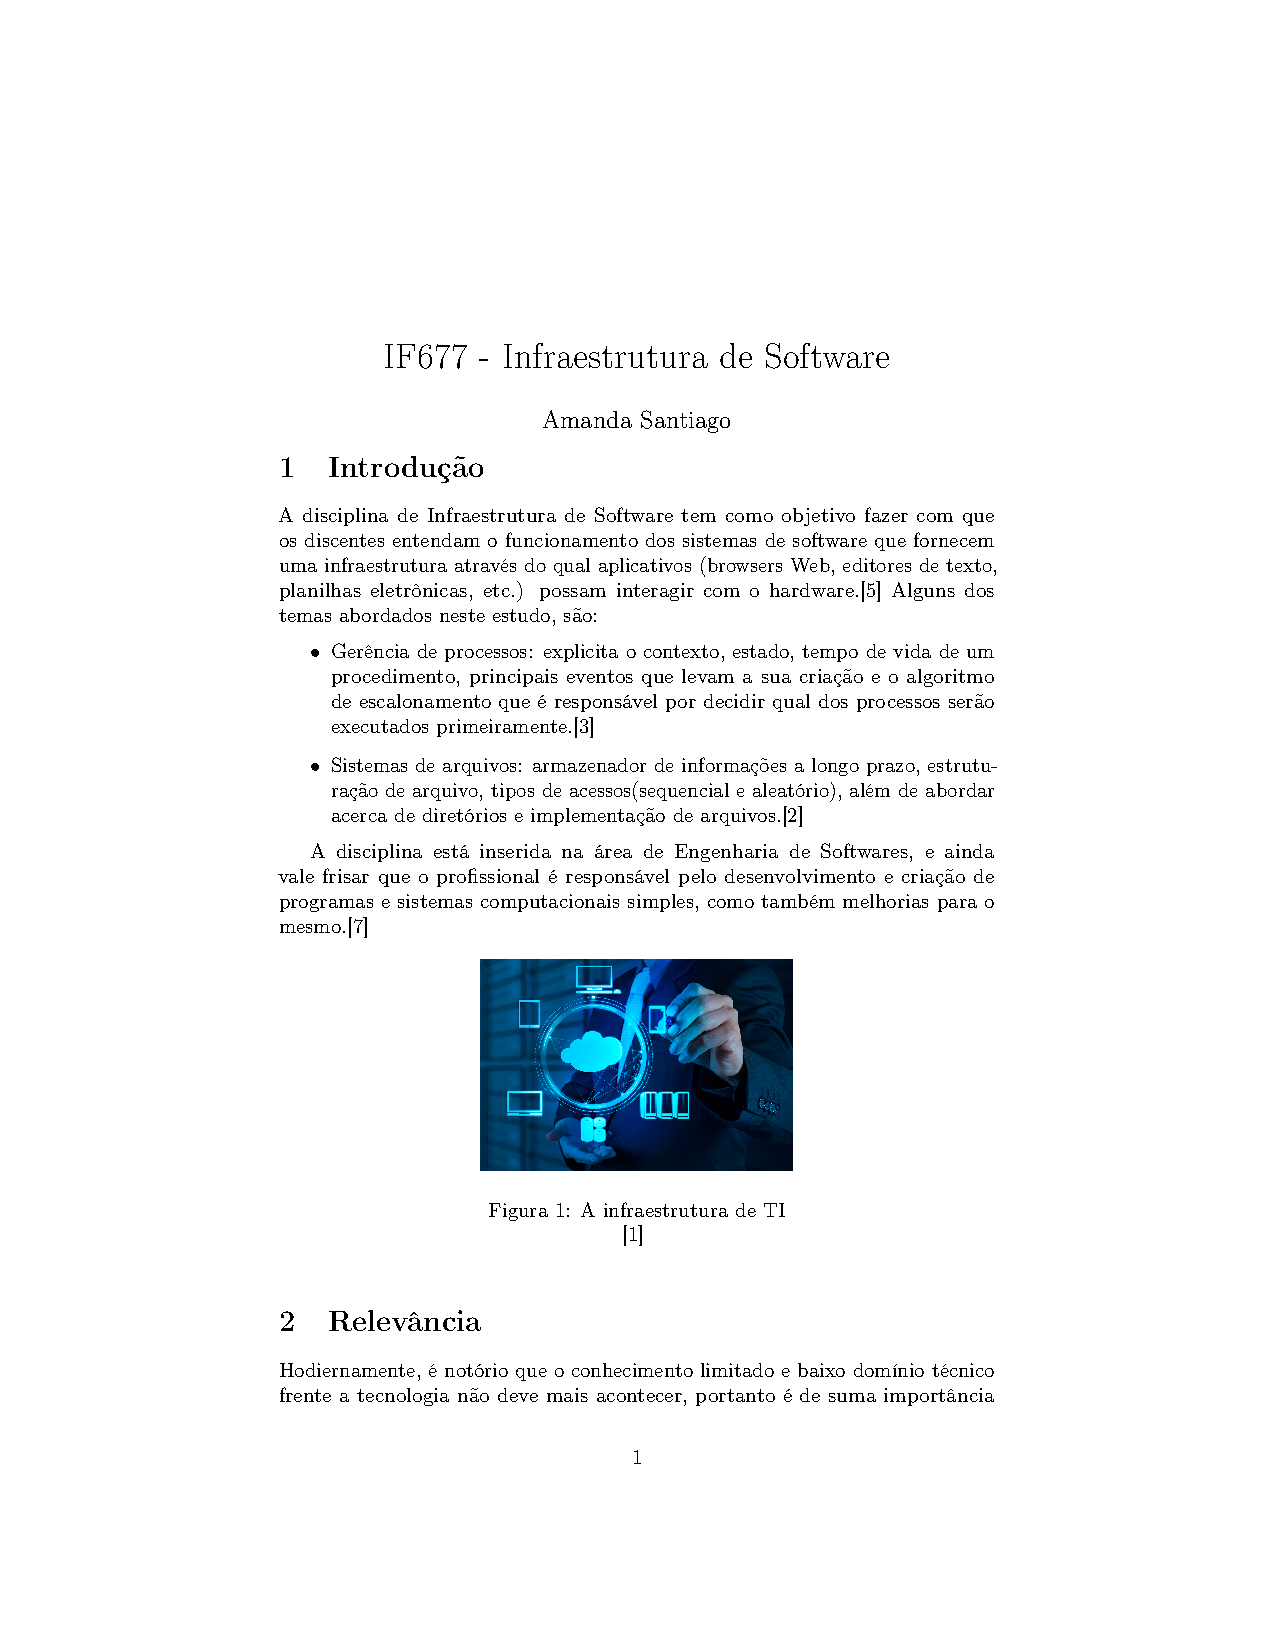
\includegraphics[scale=0.15]{ampass.png}
    \caption{A infraestrutura de TI}\cite{figura}
    \label{fig:my_label}
\end{figure}

\section{Relevância}
Hodiernamente, é notório que o conhecimento limitado e baixo domínio técnico frente a tecnologia não deve mais acontecer, portanto é de suma importância o entendimento do que permeia as relações infraestruturais de software. Da mesma maneira, a falta de competência pode gerar arquiteturas de softwares que poderão levar uma grande quantidade de sistemas a se tornarem obsoletos em pouco tempo. Por esse motivo, é crucial conhecer todos os seus componentes ou elementos, dando ênfase a parte operacional, mostrando assim sua relevância no perfil curricular do cientista da computação.\cite{fundacao}

\section{Relações interdisciplinares}


\begin{tabular}{|c|l|}

\hline

Identificação da matéria & \multicolumn{1}{c|}{Relações} \\ \hline

\begin{tabular}[c]{@{}c@{}}IF749 - Tópicos Avançados \\ em Sistemas Distribuídos\end{tabular} & \begin{tabular}[c]{@{}l@{}}Esta disciplina constitui de certa forma \\ uma complementação na formação em \\ infraestrutura de softwares,uma\\  vez que um dos principais assuntos é o\\ middleware. Por conseguinte,questões como\\ Sistemas de Arquivos Distribuídos e\\ Comunicação entre Processos estão\\ intrinsecamente ligados a esta temática.\cite{sistemas}\end{tabular} \\ \hline

\begin{tabular}[c]{@{}c@{}}IF709 - Implementação\\  Sistemas Operacionais\end{tabular} & \begin{tabular}[c]{@{}l@{}}Neste ensino, os principais objetos de estudo \\ são os conceitos básicos de sistemas \\ operacionais. É possível observar que estes \\ temas possuem relações com diversos\\  assuntos em infraestrutura de softwares, \\ a título de exemplo, tem-se: funcionalidades\\ de um sistema de arquivos, hierarquia de \\ memória, interrupções precisas e imprecisas.\cite{operacioanal}\end{tabular} \\ \hline
\end{tabular}



\bibliographystyle{plain}
\bibliography{ampass}

\end{document}
